%% Простая презентация с примером включения программного кода и
%% пошаговых спецэффектов
\documentclass{beamer}
\usepackage{fontspec}
\usepackage{xunicode}
\usepackage{xltxtra}
\usepackage{xecyr}
\usepackage{hyperref}
\setmainfont[Mapping=tex-text]{DejaVu Serif}
\setsansfont[Mapping=tex-text]{DejaVu Sans}
\setmonofont[Mapping=tex-text]{DejaVu Sans Mono}
\usepackage{polyglossia}
\setdefaultlanguage{russian}
\usepackage{graphicx}
\usepackage{listings}
\lstdefinestyle{mycode}{
  belowcaptionskip=1\baselineskip,
  breaklines=true,
  xleftmargin=\parindent,
  showstringspaces=false,
  basicstyle=\footnotesize\ttfamily,
  keywordstyle=\bfseries,
  commentstyle=\itshape\color{gray!40!black},
  stringstyle=\color{red},
  numbers=left,
  numbersep=5pt,
  numberstyle=\tiny\color{gray},
}
\lstset{escapechar=@,style=mycode}

\begin{document}
\title{EFI (и UEFI)}
\author{Свитков Сергей\\{\footnotesize\textcolor{gray}{группа 344}}}
\institute{СПбГУ}
\frame{\titlepage}

\begin{frame}\frametitle{Введение}
Что же такое EFI?
\begin{itemize}
    \item Extensible Firmware Interface 
    \item Спецификация интерфейса, разделяющего аппаратный слой и слой операционной системы
    \item Разработка Intel
    \item Используется для загрузки установленных операционных систем
    \item Пришло на замену устаревшему BIOS
    \item На самом деле, само уже успело устареть (с 2005)
\end{itemize}
\end{frame}

\begin{frame}\frametitle{Немного истории}
\begin{itemize}
    \item Первоначальные идеи возникли при разработке Intel Itanium
    \item Изначальная мотивация --- замена BIOS, обладающего тонной недостатков
    \begin{itemize}
        \item 16-bit processor mode
        \item 1MB адресуемой памяти
        \item Завязано на IBM PC/AT
    \end{itemize}
    \item Первые шаги разработки EFI были предприняты в 1998 (тогда название было иным: Intel Boot Initiative)
    \item В июле 2005 передали разработку UEFI Forum, поэтому EFI -> UEFI
    \item Последняя версия спецификации UEFI --- 2.6, январь 2016
\end{itemize}    
\end{frame}

\begin{frame}\frametitle{Преимущества по сравнению с BIOS}
\begin{itemize}
    \item Поддержка GPT, как следствие --- возможность загрузки с дисков с объемом > 2TB
    \item CPU-Independent архитектура
    \item CPU-Independent драйвера
    \item Гибкая pre-OS среда (в т.ч. поддержка связи с интернетом)
    \item Обратная совместимость
\end{itemize}
\end{frame}

\begin{frame}\frametitle{Совместимость}
Совместимость с процессорами
\begin{itemize}
    \item Itanium, x86, x86-64, ARM (AArch32), ARM64 (AArch64)
    \item В отличие от BIOS поддерживает 32 и 64 режимы
    \begin{itemize}
        \item Позволяет приложениям, работающим до загрузки системы, получать доступ ко всей памяти
    \end{itemize}
    \item Разрядность процессора и разрядность ядра должны совпадать
    \item Возможность загрузки 64-битного ядра на 32-битной реализации UEFI, запущенной на x86-64 CPU
\end{itemize}
\end{frame}

\begin{frame}\frametitle{Совместимость}
Совместимость с дисками
\begin{itemize}
    \item Поддержка и MBR и GPT
    \item MBR ограничивает количество разделов (до 4х на диске) и их размер (до 2 GB)
    \item В GPT таких ограничений нет (на самом деле есть ограничение на размер разделов до \(2 ^ {73}\) байт)
\end{itemize}
\end{frame}

\begin{frame}\frametitle{Совместимость}
Совместимость с Linux
\begin{itemize}
    \item Поддержка GPT осуществляется включением опции CONFIG\_EFI\_PARTITION при настройке ядра
    \item Можно использовать GPT и в BIOS-based системах с помощью BIOS-GPT (в GRUB 2)
    \item При желании можно добиться этого и в GRUB, но не будем об этом (Серьезно, кто использует первый GRUB в 2017?)
    \item UEFI-системы могут использовать UEFI-методы загрузки, в таком случае загрузка осуществляется с ESP 
    \item Для обратной совместимости есть поддержка MBR
\end{itemize}
\end{frame}

\begin{frame}\frametitle{Совместимость}
Совместимость с windows
\begin{itemize}
    \item Есть поддержка начиная с Windows Vista
\end{itemize}
\end{frame}

\begin{frame}\frametitle{Features}
Сервисы
\begin{itemize}
    \item Определяются два типа сервисов:
    \begin{itemize}
        \item boot services: доступны только до тех пор, пока аппаратный слой управляет платформой. Включают поддержку терминалов, а так же сервисы шины, блокировки и файлов
        \item runtime services: доступны при работе ОС; включают сервисы даты, времени и доступ к NVRAM
    \end{itemize}
    \item Variable services: предоставляют возможность сохранения данных, которые могут быть использованы и ОС и железом
    \item Time services: предоставляют поддержку временных зон, что позволяет установить аппаратные часы на UTC или локальное время
\end{itemize}
\end{frame}

\begin{frame}\frametitle{Features}
Приложения
\begin{itemize}
    \item Перед загрузкой ОС UEFI может запускать UEFI-приложения.
    \item Например, загрузчики ОС: refind, GRUB (GRUB 2), systemd-boot
    \item Можно предоставить возможность запуска других приложений
\end{itemize}
\end{frame}

\begin{frame}\frametitle{Features}
Протоколы
\begin{itemize}
    \item Поддерживает набор протоколов для коммуникации
    \item UEFI-драйвера должны предоставлять сервисы с помощью протоколов
\end{itemize}
Драйвера устройств
\begin{itemize}
    \item Помимо стандартных драйверов, специфичных для архитектуры, EFI предоставляет CPU-Independent драйвер устройства
    \item Хранится в памяти в EBC (EFI Byte Code)
    \item Можно поддерживать и специфичные для архитектуры драйвера, это позволит использовать графику/интернет до загрузки ОС-драйверов
\end{itemize}
\end{frame}

\begin{frame}\frametitle{Features}
Взаимодействие между EFI-bootmanager'ом и EFI-драйверами
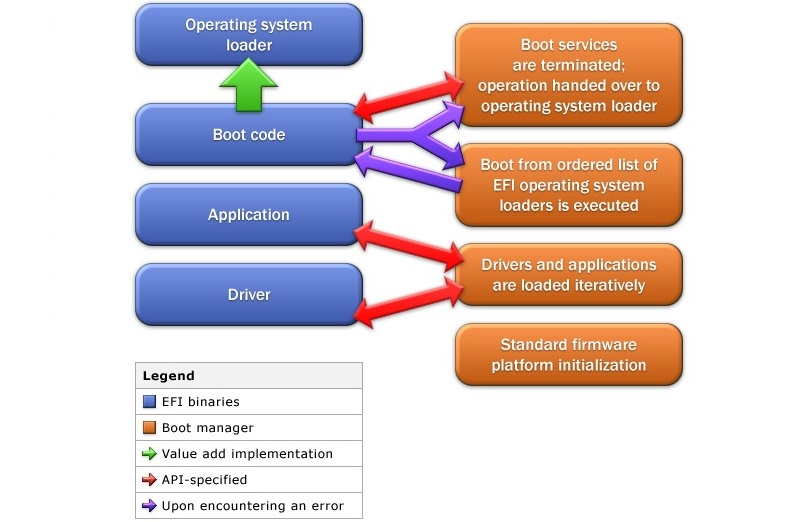
\includegraphics[width=\textwidth,height=\textheight,keepaspectratio]{pics/Efi_flowchart_extended.jpg}
\end{frame}

\begin{frame}\frametitle{Features}
Графика
\begin{itemize}
    \item EFI использовало UGA-протокол (Universal Graphic Adapter) для поддержки графики
    \item UEFI использует Graphics Output Protocol с целью избавиться от зависимости от VGA
    \item Большинство ранних реализаций были основаны на CLI, но с 2007 появилась поддержка GUI
\end{itemize}
\end{frame}

\begin{frame}\frametitle{Features}
EFI system partition
\begin{itemize}
    \item Хранит UEFI-applications и файлы, которые нужны приложениями (например, ядро вашего дистрибутива)
    \item В качестве ФС используется специальная версия FAT
    \item Есть место для boot-sector для обратной совместимости с BIOS
\end{itemize}
\end{frame}

\begin{frame}\frametitle{Features}
Загрузка
\begin{itemize}
    \item UEFI-booting
    \begin{itemize}
        \item Использует не boot sector, а boot manager
        \item Автоматически распознает загрузчики ОС
    \end{itemize}
    \item CSM (Compability Support Module) booting --- для обратной совместимости 
    \item Network booting
    \item Secure boot
    \begin{itemize}
        \item Специальный протокол, который не позволяет загружаться драйверам или загрузчикам ОС с неподходящей сигнатурой
    \end{itemize}
\end{itemize}
\end{frame}

\begin{frame}\frametitle{Features}
UEFI shell
\begin{itemize}
    \item Shell environment
    \item Позволяет запускать различные UEFI-приложения
    \item Может быть полезен для исправления/диагностики проблем с загрузчиками
\end{itemize}
\end{frame}

\end{document}